\documentclass[a4paper,11pt]{article}
\usepackage[utf8]{inputenc}
\usepackage{graphicx}
\usepackage{subcaption}
\usepackage{chngcntr}
\counterwithin{figure}{section}
\usepackage{authblk}
\usepackage{titling}
\setlength{\droptitle}{-10em}   % This eliminates the space on top of title
\usepackage[font=scriptsize]{caption}
\usepackage{float}

%opening
\title{Intelligent Systems Homework 2}
\author{Akhil Kanna Devarashetti}
\begin{document}
\affil{M13471127}
\maketitle

\begin{abstract}
This homework deals with the predication of a disease based on two parameters L and P. Three models are used to predict the disease namely K-Nearest Neighbours, Neighbourhood and Perceptron. Each algorithm is studied to decide the optimal hyper-parameter values. Finally, the performance of each algorithm is analyzed.
\end{abstract}

\section{KNN and Neighbourhood Classifiers}
\subsection{k Nearest Neighbours Classifier}
I ran the k-Nearest Neighbours algorithm with the k values from 1 to 31 in odd numbers for the scaled data. For all the algorithms in this article, the data has been scaled from 0 to 1 for each attribute. From the hit-rate graph obtained as shown in Fig. \ref{fig:1.1a}, I observed that the hit-rate was maximum when the value of k is 15. So I recommend using 15 as k for the given data.

\begin{figure}[ht]
    \centering
    \begin{subfigure}[b]{0.49\linewidth}
        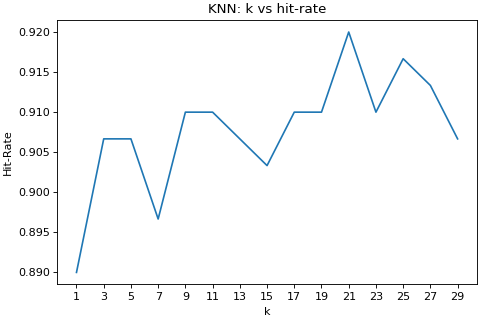
\includegraphics[width=\linewidth]{knn.png}
        \caption{Hit-rate for different values of k}
        \label{fig:1.1a}
    \end{subfigure}
    \begin{subfigure}[b]{0.49\linewidth}
        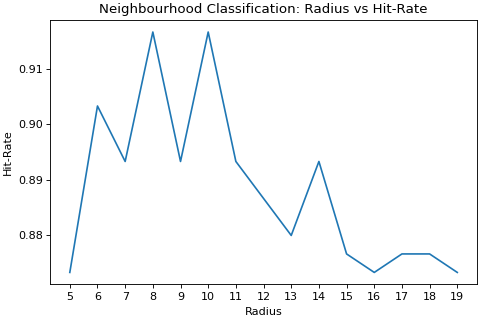
\includegraphics[width=\linewidth]{neighbourhood.png}
        \caption{Hit-rate for different values of radius}
        \label{fig:1.1b}
    \end{subfigure}
    \caption{}
\end{figure}

\subsection{Neighbourhood Classifier}
For the neighbourhood algorithm, I ran the scaled data 14 times with radius from 0.05 to 0.7. Based on the hit-rate observed as shown in Fig. \ref{fig:1.1b}, the maximum hit-rate occurred when the radius is 0.15, so I recommend choosing the 0.15 as the best radius for this algorithm.

\newpage
\section{Perceptron Classifier}
For my perceptron algorithm, I initially started with 100 epochs with a learning rate of 0.001 and figured out with a few trails that the model is classifying sufficiently good with 40 epochs on 0.01 learning rate. The learning (change of weights) happens for every data point. I experimented with the initialization of weights by first choosing all 0s, random floating point numbers from -10 to 10, 0 to 10, 0 to 1 and -1 to 1. It turns out that for all my trails, the weights would converge to their optimal values quickly. So, essentially, any of my tested policy would work, however, I chose the random values form -1 to 1 as the best policy because convergence was quicker than other policies. For all the experiments conducted in this problem, the data was split into 80\% for training and 20\% for testing. From the Fig. \ref{fig:2.1}, we can see that both the training and testing error drops quickly with increased epochs and the test error ends at a bit lower than the training set. However, this is not the case for random splits, the change in error may vary, but end up at a similar value after 60 epochs. Even after training the perceptron for thousands of epochs, the mean squared error of the perceptron did not go to 0 and the changes in weights became negligible. As the data given is not linearly separable, the perceptron never reaches a 0 error. Hit-rate on test set was 96.7\% with a mean squared error of around 25 on training data.

\begin{figure}[h!]
    \centering
    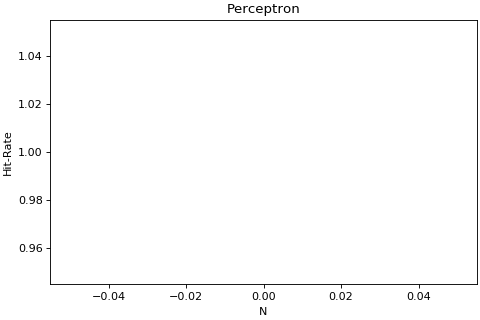
\includegraphics[width=0.7\linewidth]{perceptron.png}
    \caption{Training and testing error of perceptron for 70 epochs.}
    \label{fig:2.1}
\end{figure}

\newpage
\section{Performance Analysis}

\subsection{Performance on Individual Trials}
\begin{figure}[ht]
    \centering
    \begin{subfigure}[b]{1\linewidth}
        \includegraphics[width=\linewidth]{KNN_Classifier_metric_bars.png}
        \caption{Hit-rate for different values of k}
        \label{fig:3.1a}
    \end{subfigure}
    \begin{subfigure}[b]{1\linewidth}
        \includegraphics[width=\linewidth]{Neighbourhood_Classifier_metric_bars.png}
        \caption{Hit-rate for different values of radius}
        \label{fig:3.1b}
    \end{subfigure}
    \begin{subfigure}[b]{1\linewidth}
        \includegraphics[width=\linewidth]{Perceptron_Classifier_metric_bars.png}
        \caption{Hit-rate for different values of radius}
        \label{fig:3.1b}
    \end{subfigure}
    \caption{}
    \label{fig:3.1}
\end{figure}

\subsection{Average Performance}
\begin{figure}[H]
    \centering
    \includegraphics[width=1\linewidth]{average_performances_cropped.png}
    \caption{Training and testing error of perceptron for 70 epochs.}
    \label{fig:3.2}
\end{figure}

\subsection{Trial-Wise Training Error Time-Series for the Perceptrons}
\begin{figure}[H]
    \centering
    \includegraphics[width=0.7\linewidth]{training_error.png}
    \caption{Training and testing error of perceptron for 70 epochs.}
    \label{fig:2.1}
\end{figure}

\subsection{Mean Training Error for the Perceptron}
\begin{figure}[H]
    \centering
    \includegraphics[width=0.8\linewidth]{mean_training_error.png}
    \caption{Training and testing error of perceptron for 70 epochs.}
    \label{fig:2.1}
\end{figure}

\subsection{Best k-NN Decision Boundary}
\begin{figure}[H]
    \centering
    \includegraphics[width=0.6\linewidth]{knn_decision_boundary.png}
    \caption{Training and testing error of perceptron for 70 epochs.}
    \label{fig:2.1}
\end{figure}

\subsection{Best Neighborhood Classifier Decision Boundary}
\begin{figure}[H]
    \centering
    \includegraphics[width=0.6\linewidth]{neighbourhood_decision_boundary.png}
    \caption{Training and testing error of perceptron for 70 epochs.}
    \label{fig:2.1}
\end{figure}

\subsection{Perceptron Decision Boundary}
\begin{figure}[H]
    \centering
    \includegraphics[width=0.5\linewidth]{perceptron_decision_boundary.png}
    \caption{Training and testing error of perceptron for 70 epochs.}
    \label{fig:2.1}
\end{figure}

\begin{figure}[h!]
    \centering
    \includegraphics[width=0.4\linewidth]{scatter.png}
    \caption{Training and testing error of perceptron for 70 epochs.}
    \label{fig:3.8}
\end{figure}

\subsection{Analysis of Results}
\subsubsection{Suitability of the classifiers}
From Figure \ref{fig:3.8}, we can notice that the data points form circular looking shapes for each class next to one another. In general, when the data is spread in such a form, the kNN and Neighbourhood classifiers tend to perform with high accuracy and are fairly suitable. The data can be clearly seen as not linearly separable. However, majority of the points of both classes lie in different regions which is usually good for linear-fit models like perceptron.

For the 9 trails conducted shown in Figure \ref{fig:3.1} and Figure \ref{fig:3.2}, it appears that kNN classifier is most suitable as it outperforms neighbourhood classifier on Sensitivity, NPV and hit-rate. However kNN performs only marginally better than perceptron algorithm on specificity, PPV and hit-rate. On the other hand, neighbourhood classifier gave better specificity and PPV values compared to perceptron.

\subsubsection{Pros and Cons of the classifiers}
Pros of kNN and Neighbourhood:
\begin{itemize}
  \item They both do not need any prior learning. But the cost of classifying a data point is high because it requires distances to be calculated between the new data point and all the other points in the training set. However this can be reduced by calculating distances of only those points within a boundary of standard deviation and multiples of it.
  \item These algorithms can be a good base line models to validate much complex models like neural networks or decision trees.
\end{itemize}
Cons:
\begin{itemize}
  \item Neighbourhood classifier would not classify a new data point if there are no data points within the fixed radius. We can overcome this easily by tweaking it to act like a kNN classifier at that moment with k = 1.
  \item There is no decision boundary function which we could take leverage of.
\end{itemize}
Pros of Perceptron:
\begin{itemize}
  \item Cost of classifying a new data point is lower than the other two classifiers.
  \item If combined with more perceptrons in layers, the model could classify non-linear decision boundaries which could be more powerful than the other two classifiers.
\end{itemize}
Cons:
\begin{itemize}
  \item Training the model requires trial and error.
  \item Training itself will take long.
  \item Will not classify properly if the data is not remotely close to linearly separable.
\end{itemize}

\subsubsection{Deciding the best classifier}
As there is no urgency to know whether the patient is diseased or not and that the accuracy of the classification is vital for the patient, I would consider getting a better classification, even if it takes a bit longer to do so. As the kNN classifier performed better than the other two classifiers in my 9 trails, I would recommend using kNN classifier for this problem.

\end{document}